\chapter{Telecomunicacion network basics}
\section{The OSI and Internet models}

L'architettura \textbf{Open System Interconnetion(OSI)} punta a collegare sistemi
eterogenei fra di loro, la sua specifica è la \textbf{ISO 7498} ed è un modello
costituito di 7 \textit{strati}.

\begin{figure}[!ht]
	\centering
	% TODO: ingrandire immagine a 0.4
	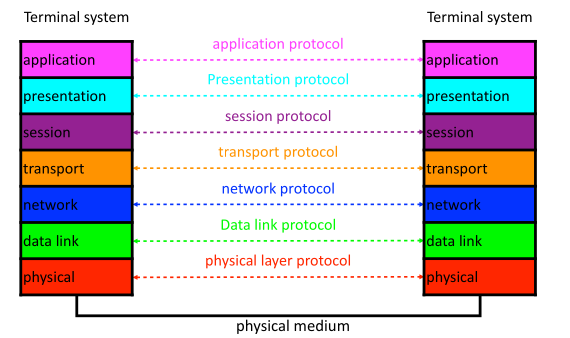
\includegraphics[width=0.4\columnwidth]{./images/osi.png}
	\caption{Architettura OSI}
	\label{fig:osi}
\end{figure}

\subsection{Application Layer}
Livello del modello OSI dove le applicazioni accedono ai servizi di rete, permette ad esempio
di trasferire un file, connettersi a database, uso di mail, ecc.

\subsection{Presentation Layer}
Livello del modello OSI adibito alla trasmissione di dati, traduce differenti formati di dati 
presenti nell'Application Layer in uno standard per gli strati inferiori.

Fornisce servizi per la trasmissione sicura ed efficiente dei dati come:
\begin{itemize}
  \item data encryption
  \item data compression
  \item altre
\end{itemize}

\subsection{Session Layer}

Livello del modello OSI che permette due computer diversi di \textbf{creare}, \textbf{usare}
e \textbf{finire} una sessione, utile per trasmissione di dati e accesso in remoto.

Introduce:
\begin{itemize}
  \item \textbf{Controllo di dialogo}: per regolare la trasmissione e la durata delle stesse
  \item \textbf{Gestione dei token e sincronizzazione}
\end{itemize}

\subsection{Transport Layer}
Livello del modello OSI adibito alla gestione dei pacchetti da trasmettere:
\begin{itemize}
  \item Divide pacchetti grandi in più piccoli
  \item Riordina i pacchetti nell'ordine correto all'arrivo
\end{itemize}

Gestisce inoltre il riconoscimento degli errori e il loro recupero:
\begin{itemize}
  \item Ricezzione di pacchetti di confermo dell'arrivo (ACK)
  \item Reinvia pacchetti persi
\end{itemize}


\subsection{Network Layer}
Livello del modello OSI adibito alla gestione dell'instradamento dei dati attraverso le sottoreti:
\begin{itemize}
  \item Determina il percorso di instradamento per arrivare alla destinazione
  \item gestisce problemi di congestione
\end{itemize}


\subsection{Data Link Layer}
Impacchetta bits in frames per il layer fisico, provvede a fornire un metodo di trasmissione dei frames affidabile.


\subsection{Physical Layer}
Trasmette bits da pc a pc, regola la trasmissione dello stream di bits sul mezzo fisico.

Definisce come i cavi sono collegati ai pc, come i segnali sono codificati e come i cavi sono collegati ai pc.


\subsection{Servizi del sistema OSI}
Nel sistema OSI ogni layer fornisce un servizio al layer superiore e consuma il servizio del layer inferiore.

Gli strati posono offrire servizi connessioneless o connection-oriented.

Gli strati possono fornire servizi affidabili per evitare la perdita di dati o non affidabili.

I \textbf{Service} è il set di primite fornite da un layer ad un'altro layer e definisce cosa un layer è capace di fare.


\textbf{Protocol} è un set di regole che definisce il formato e il significato dei messaggi scambiati tra entità del livello.

\subsection{Internet Protocol Vs OSI}

L'internet protocol è formato di 7 strati, il modello OSI è formato di 4 strati(perchè tcp e ip sono unificati in un unico livello):
\begin{itemize}
  \item \textbf{Application}: Application, Presentation, Session
  \item \textbf{TCP(reliable)/UDP(non reliable)}: Transport
  \item \textbf{IP}: Network
  \item \textbf{Network Access}: Data Link, Physical
  \item \textbf{Hardware}: Physical
\end{itemize}

\section{Communication models}
Le tipologie di comunicazione sono dipendenti dalle entità coinvolte:
\begin{itemize}
  \item \textbf{end-to-end e relayed}: location
  \item \textbf{unicast, multicast, broadcast}: comunicazione tra una sorgente e un gruppo di destinazioni(number)
  \item \textbf{client-server, peer-to-peer}: comunicazione tra un server e un client o tra due entità terminali(role)
\end{itemize}







\section{Delimitation}



Delimita le Unita Informative(UI o in inglese IU) da trasmettere in bit o byte, step necessario per permettere ai layer sottostanti di trasmettere i dati.

Implementa metodi per delimitare le UI:
\begin{itemize}
  \item bit/byte counting
  \item inserimento di start e stop bit
\end{itemize}

\subsection{Bit/Char stuffing}
Dopo una ripetizione di un valore binario per 5 volte, si aggiunge un valore opposto per delimitare la UI.
Esempio: Avendo una UI $0000000000$, si aggiunge un 1 per delimitare la UI e diventa $000001000001$.

I vantaggi introdotti sono quelli inerenti alla robustezza e alla sincronizzazione.
Mentre gli svantaggi sono legati alla ridondanza delle informazioni e alla perdita di efficienza.





\section{Sequence control}

\subsection{Fragmentation and aggregation}
Capacità di dividere dati in blocchi più piccoli per la trasmissione e di aggregare più blocchi in un unico blocco.


\subsection{Risequentialization}
Necessaria per riordinare i pacchetti nell'ordine corretto all'arrivo.



\section{Error management}

Il controllo dell'errore ha 3 possibili soluzioni:
\begin{itemize}
	\item \textbf{Error detection}: rilevazione dell'errore
	\item \textbf{Error correction}: correzione dell'errore
	\item \textbf{Error recovery}: recupero dell'errore
\end{itemize}
\subsection{Error Detection}


La error detection si ottiene mediante l'aggiunta di ridondanza ai dati da trasmettere come ad esempio il parity check, aggiunge un bit a $1$ se la sequenza ha un numero dispari di $1$ e $0$ se la sequenza ha un numero pari di $1$.


Se applicato questo processo ad un blocco di 2 dimensioni si ottiene la block parity check, che permette di rilevare errori.

\begin{figure}[!ht]
  \begin{adjustbox}{width=0.5\columnwidth, center}
    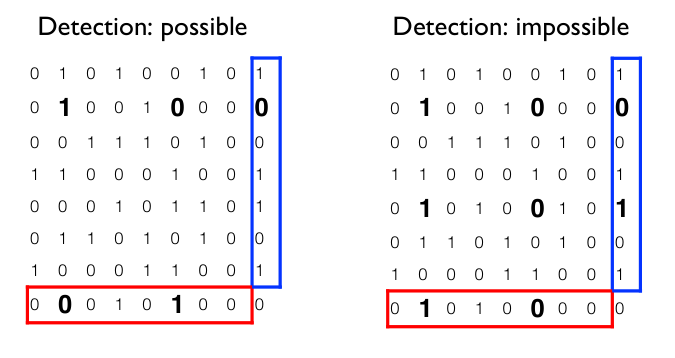
\includegraphics{images/parity_block.png}
    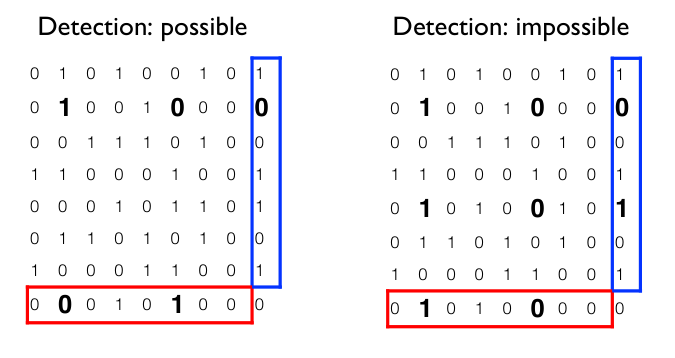
\includegraphics{./images/parity_block.png}
  \end{adjustbox}
    \caption{Parity block}
    \label{fig:parity_block}
\end{figure}


\subsection{Complement sum}

\begin{figure}[!ht]
	\centering
	% TODO: ingrandire immagine a 0.4
	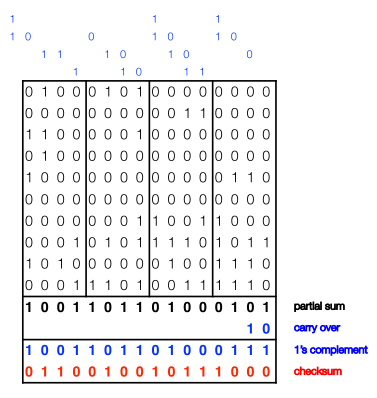
\includegraphics[width=0.4\columnwidth]{./images/complement_sum.png}
	\caption{Complement sum}
	\label{fig:complement_sum}
\end{figure}

Quando si riceve il pacchetto, si calcola il \textbf{checksum} dei dati ricevuti(come in \autoref{fig:complement_sum})
e lo si confronta al checksum allegato al pacchetto ricevuto,
nel caso di checksum differente si deve ritrasmettere il pacchetto.

\subsubsection{Other codes}

\textbf{Polynomial codes} conosciuti anche come \textbf{Cyclic Redundancy Check(CRC)},
usano moltiplicazioni tra polinomi per effettuare il checksum.



\subsection{Error Correction}



Con la \textbf{block parity check} si possono recuperare errori ma solo se presente un errore di 1 bit.

Vengono quindi introdotte tecniche \textbf{Forward Error Correction(FED)}(\href{https://en.wikipedia.org/wiki/Viterbi_algorithm}{ad esempio Algoritmo di Viterbi})
che permettono di capire la presenza di un errore mediante algoritmi di ricostruzione.

Con FED si ricorre a ridondanza per eliminare errori(pochi in numero), non sono necessari messaggi
di corretta ricezione, che torna molto utile nel caso di comunicazione unidirezionale.


\begin{figure}[!ht]
	\centering
	% TODO: ingrandire immagine a 0.4
	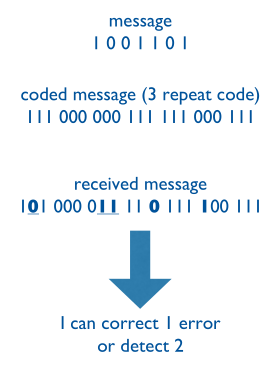
\includegraphics[width=0.4\columnwidth]{./images/repetition_code.png}
	\caption{Repetition code}
	\label{fig_repetition_code}
\end{figure}


\subsection{Error Recovery}
Quando si parla di comunicazione in reti di comunicazioni, si ricade nel richiedere automaticamente
un pacchetto che non risulta corretto al ricevitori,
esistono approcci automatici come \textbf{Automatic Repeat Request, ARQ}.

Esistono inoltre differenti meccanismi di ritrasmissione che come punto focale hanno:
\begin{itemize}
	\item Error detection
	\item Acknowledgements
	\item timers
	\item IU identifiers
\end{itemize}


Le procedure ARQ cambiano in base alla dimensione delle finestra:
\begin{itemize}
	\item \textbf{Stop and wait}: finestra di dimensione 1, si attende l'ack prima di inviare il pacchetto successivo
	\item \textbf{Sliding window, go-back-N}: finestra di dimensione N, si inviano N pacchetti prima di attendere l'ack(non ha un selettore per il resending e invia tutto il blocco)
	\item \textbf{Sliding window, selective repeat}: finestra di dimensione N, si inviano N pacchetti prima di attendere l'ack(ha un selettore per il resending e invia solo il pacchetto corrotto)
\end{itemize}


\subsubsection{Stop and Wait}

Il pacchetto \textbf{ACK(acknowledgement)} solitamente è molto corto per evitare
correzzioni nel pacchetto che conferma la corretta ricezione.

È necessario stabilire un tempo limite entro il quale si da per scontato
la \textit{scomparsa} del pacchetto, solitamente si basa sul \textbf{Round Trip Time(RTT)} che
dipende dalla congestione  della rete e ne misura i ritardi per arrivare da punto A a punto B.

Altro fattore chiave è capire quali dati sono stati inviati e quali no, per evitare
duplicazioni.
Per questo problema di è scelto di indicizzare i pacchetti con una sequenza che prende
il nome di \textbf{SeQuence Number(SQN)} per identificare univocamente quali pacchetti da ritrasmettere.

Si può parlare anche di ACK comulativi mediante l'uso di SQN consecutivi.

\begin{figure}[!ht]
	\centering
	% TODO: ingrandire immagine a 0.4
	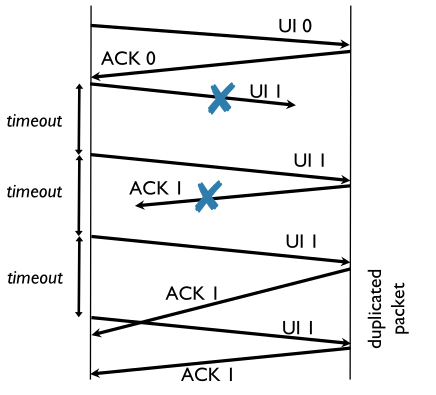
\includegraphics[width=0.4\columnwidth]{./images/esempio_comunicazione_stop_wait_no_sqn.png}
	\caption{Esempio comunicazione stop and wait senza SQN}
	\label{fig:esempio_comunicazione_stop_wait_no_sqn}
\end{figure}


\begin{figure}[!ht]
	\centering
	% TODO: ingrandire immagine a 0.4
	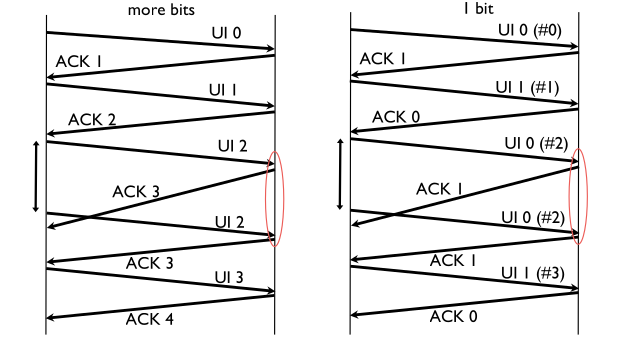
\includegraphics[width=0.4\columnwidth]{./images/esempio_comunicazione_stop_wait_sqn.png}
	\caption{Esempio comunicazione stop and wait con SQN}
	\label{fig:esempio_comunicazione_stop_wait_sqn}
\end{figure}



\subsubsection{Stop and wait performance}

I tempi considerati sono:
\begin{itemize}
	\item \textbf{$T_U$}: tempo di trasmissione di un pacchetto, misurato in $s/IU$
	\item \textbf{$T_P$}: tempo di propagazione di un pacchetto, misurato in $s/IU$
	\item \textbf{$T_{A}$}: tempo di trasmissione di un ACK, misurato in $s/IU$
\end{itemize}

Il tempo totale per inviare un'unità informativa(caso ideale):
\begin{align}
	T_{tot} = T_{U} + 2T_{P} + T_{A}
\end{align}

Il massimo grado di utilizzo di un canale di comunicazione nel caso di \textbf{assenza di errore}:
\begin{align}
	\rho_0
	 & =\frac{T_U}{T_{tot}}                                                     \\
	 & = \frac{T_U}{T_U + 2T_P + T_A}                                           \\
	 & = \begin{cases}
		     \frac{1}{2 + 2 \frac{T_P}{T_U}} \quad \text{se}\quad T_U = T_A  \\
		     \frac{1}{2 \frac{T_P}{T_U} + 1} \quad \text{se}\quad T_U >> T_A \\
		     0 \quad \text{se}\quad T_P >> T_U
	     \end{cases}
\end{align}



Nel caso di \textbf{presenza di errore}, non viene ricevuto l'ACK dal trasmettitore, devo fare alcune assunzioni:
\begin{itemize}
	\item Indipendenza statisticamente dei pacchetti informativi
	\item perdita di pacchetti ACK
\end{itemize}

Indico con $p$ la probabilità di perdita del pacchetto.


Il tempo per l'arrivo di un pacchetto con presenza di errori diventa:
\begin{align}
	\Bar{T_1} = & (N_t - 1) T_0 + T_1     \\
	=           & \frac{p}{1-p} T_0 + T_1 \\
	\simeq      & \frac{T_1}{1-p}
\end{align}

Dove $N_t$ è desscritta come:
\begin{align}
	N_t = \sum_{k=1}^{\infty} k p^{k-1} (1-p) = \frac{1}{1-p}
\end{align}

Quindi l'utilizzazione del canele diventa:
\begin{align}
	\rho = (1 - p) \rho_0
\end{align}


\subsubsection{Sliding window}
La ricezione con \textbf{sliding window} può essere non sequenziale ma non può superare il \textbf{timeout} che invalida il pacchetto.

Esistono due strategie per il reinvio dei dati persi con la tecnica dello sliding window:
\begin{itemize}
  \item \textbf{go-back-N}: torna indietro di un numero $N$ di unità informative
  \item \textbf{selective repeat}: reinvia solo i pacchetti effetivamnete persi
\end{itemize}

\begin{figure}[!ht]
	\centering
	% TODO: ingrandire immagine a 0.4
	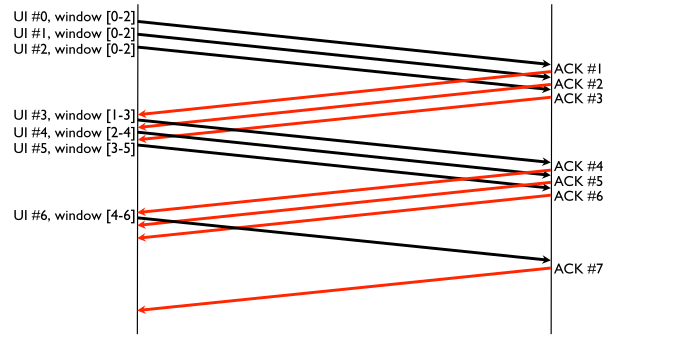
\includegraphics[width=0.4\columnwidth]{./images/sliding_window_base.png}
  \caption{Sliding window base}
  \label{fig:sliding_window_base}
\end{figure}


\begin{figure}[!ht]
	\centering
	% TODO: ingrandire immagine a 0.4
	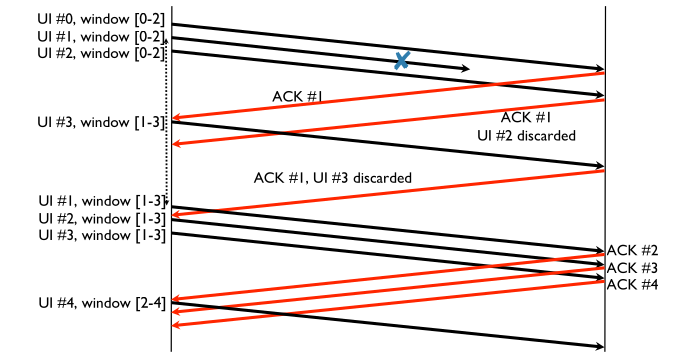
\includegraphics[width=0.4\columnwidth]{./images/sliding_window_go_back_n.png}
  \caption{Sliding window go back N}
  \label{fig:sliding_window_go_back_n}
\end{figure}

\begin{figure}[!ht]
	\centering
	% TODO: ingrandire immagine a 0.4
	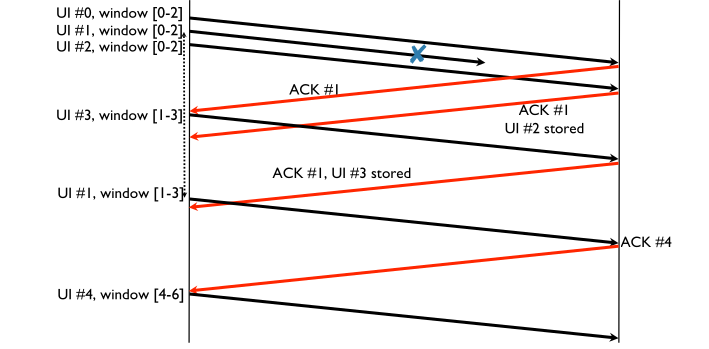
\includegraphics[width=0.4\columnwidth]{./images/sliding_window_selective_repeat.png}
  \caption{Sliding window selective repeat}
  \label{fig:sliding_window_selective_repeat}
\end{figure}



